\documentclass[12pt]{article}
\usepackage[spanish,mexico]{babel}
	\selectlanguage{spanish}
\usepackage{graphicx}
\usepackage{amsmath}
\usepackage{wrapfig}
\usepackage[dvipsnames]{xcolor}
\usepackage{float}
\usepackage{multicol}
\usepackage{geometry}
\usepackage{hyperref}
\usepackage[utf8]{inputenc}

\newgeometry{top=2cm}

\title{Actividad 7: Espacio Fase}
\author{Paulina Valenzuela Coronado}
\date{Marzo de 2016}

\begin{document}
\maketitle
\section{Introducción}
Un péndulo simple está constituido por un hilo inextensible de masa despreciable, sostenido por su extremo superior de un punto fijo, con una masa puntual sujeta en su extremo inferior que oscila libremente en un plano vertical fijo.
El movimiento solo ocurre en dos dimensiones y este no pierde energía por la fricción o la resistencia del aire.\cite{Wiki} \\

La ecuación del movimiento de un péndulo simple es 

\begin{equation}
	\frac{
		d^2\theta}{dt^2}+\frac{g}{l}\sin\theta=0
\end{equation}

donde
\begin{itemize}
	\item $g$ es la aceleración debida a la gravedad
	\item $l$ es el lago del péndulo
	\item $\theta$ es el desplazamiento angular 
\end{itemize}


El \textbf{espacio fase} es una representación geométrica de todas las trayectorias de un sistema dinámico no plano. Cada curva representa una condición inicial diferente. Un retrato de fase es una herramienta valiosa en el estudio de los sistemas dinámicos autónomos de segundo orden. La configuración de las curvas en el espacio de fase revela información sobre la existencia de atractores, repulsores, ciclos límite, entre otras cosas. Cada línea mostrada en el espacio fase representa un par de condiciones iniciales, al ser una solución cíclica, se forman círculos en lugares donde las condiciones son estables y líneas onduladas no cerradas cuando las condiciones iniciales no propician un lugar de equilibrio para el sistema. \cite{E} \\

En esta actividad usamos la herramineta \textit{scipy.integrate.odeint}, que utilizamos en la actividad 5, para resolver las ecuaciones diferenciales ordinarias, esta herramienta las transforma en ecuaciones de primer orden por medio de un cambio de variable. De esta manera, es más fácil obtener una solución numérica para la ecuación.  \cite{Spicy}

\section{Programa: Espacio fase de un péndulo simple.}

Se presenta a continuación el código realizado. 

\begin{verbatim}
import numpy as np
from scipy.integrate import odeint
import matplotlib.pyplot as p

#Condiciones iniciales
b = 0 
g = 9.8
l = 1.0
c = g/l


def pend(y, t, b, c):
theta, omega = y
dydt = [omega, -b*omega - c*np.sin(theta)]
return dydt


y0 = np.array([-4*np.pi, 4*np.pi])
y1 = np.array([-2*np.pi, 0*np.pi])
t = np.linspace(0, 10, 101)

values  = linspace(-1,1, 50)                          # position of X0 between X_f0 and X_f1
vcolors = p.cm.autumn_r(linspace(0.3, 1., len(values)))  # colors for each trajectory


#-------------------------------------------------------
# plot trajectories
for v, col in zip(values, vcolors):
x0 = v * y0                                  # starting point
x1 = v * y1
x = odeint(pend, x0, t, args=(b,c))         #Calcula la ecuación diferencial
p.plot( x[:,0], x[:,1], lw=3.5*v, color=col, label='x0=(%.f, %.f)' % ( x0[0], x0[1]) )
xp = odeint(pend, x1, t, args=(b,c))         #Calcula la ecuación diferencial
p.plot( xp[:,0], xp[:,1], lw=3.5*v, color=col, label='x1=(%.f, %.f)' % ( x1[0], x1[1]) )

#-------------------------------------------------------

#-------------------------------------------------------
# I choose to plot normalized arrows and to use colors to give information on
# the growth speed
p.title('Espacio Fase')
p.xlabel('Angulo')
p.ylabel('Velocidad Angular')
p.xlim(-2*np.pi,2*np.pi)
p.ylim(-10,10)
p.grid()
\end{verbatim}

\begin{figure}[H]
\centering
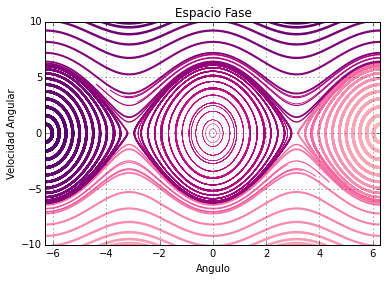
\includegraphics[width=16cm]{3.png}
\caption{Espacio fase generado para las condiciones iniciales}
\end{figure}

\pagebreak

\begin{thebibliography}{6}
	
	\bibitem{Wiki}
	Wikipedia en Español, https://es.wikipedia.org/wiki/P%C3%A9ndulo
	\emph{Péndulo}
	\bibitem{Spicy}
	http://docs.scipy.org/doc/scipy/reference/integrate.html
	
	
	\bibitem{E}
	Wikipedia,
	\emph{Retrato de fase}. Recuperado en marzo de 2016 de \url{https://es.wikipedia.org/wiki/Retrato_de_fase}


\end{thebibliography}

\end{document}
